\documentclass[12pt]{article}

\usepackage{algorithm}
\usepackage[noend]{algorithmic}
\usepackage{amsmath}
\usepackage[italian]{babel}
\usepackage{caption}
\usepackage{enumitem}
\usepackage{float}
\usepackage{fullpage}
\usepackage{graphicx}
\usepackage[colorlinks=true, urlcolor=blue]{hyperref}
\usepackage[utf8]{inputenc}
\usepackage{minted}
\usepackage{subcaption}
\usepackage{tabularx}

% Hacks needed to get the algorithm package to work as intended.
\floatname{algorithm}{Algoritmo}
\renewcommand{\algorithmicrequire}{\textbf{Input:}}

\title{Progetto del corso Sistemi Distribuiti: Paradigmi e Modelli, 2012/2013}
\author{
	Jacopo Notarstefano\\
	\texttt{jacopo.notarstefano [at] gmail.com}
}
\date{}

% http://tex.stackexchange.com/a/4304/10806
\newcommand{\cpp}{C\nolinebreak\hspace{-.05em}\raisebox{.4ex}{\tiny\bf +}\nolinebreak\hspace{-.10em}\raisebox{.4ex}{\tiny\bf +}}
\newcommand{\mpp}{Magick\nolinebreak\hspace{-.05em}\raisebox{.4ex}{\tiny\bf +}\nolinebreak\hspace{-.10em}\raisebox{.4ex}{\tiny\bf +}}

\begin{document}
  \maketitle
    \section{Introduzione}

    Scopo di questo progetto è dare un'implementazione sequenziale e una
    parallela di una soluzione al problema dell'Histogram Thresholding, per
    poi confrontarne le performance sia fra esse sia con i modelli teorici.

    Entrambe le implementazioni sono realizzate in \cpp; in particolare
    quella parallela è data in termini di parallel skeleton, più nello
    specifico quelli forniti dal framework 
    \href{http://sketo.ipl-lab.org/}{\underline{SkeTo}}.

    SkeTo è uno skeleton framework in cui dichiarazione e istanziazione degli
    skeleton avvengono allo stesso tempo. I metodi offerti dalle classi
    astratte del framework, implementate in termini di template, sono quelli
    tipici della programmazione funzionale, come \texttt{map}, \texttt{reduce}
    e \texttt{scan}. Queste caratteristiche rendono molto compatto il codice:
    in effetti l'intero codice non funzionale parallelo di
    \texttt{src/parallel.cpp} ammonta a \(63\) righe commenti inclusi, di cui
    appena \(3\) chiamate di libreria.

    Il codice non funzionale sequenziale di \texttt{src/sequential.cpp} \`e
    un ordinario programma \cpp. La struttura delle due implementazioni \`e
    molto simile: questo perch\'e il business code dell'applicazione \`e
    stato incapsulato nella classe \texttt{Job}, la cui interfaccia \`e
    definita in \texttt{src/job.h} e la cui implementazione in
    \texttt{src/job.cpp}.

    Per prima cosa presentiamo il problema dell'Histogram Thresholding e
    descriviamo l'algoritmo risolutivo implementato. In seguito descriviamo in
    maggiore dettaglio le scelte implementative adottate durante lo sviluppo.
    Parte centrale del lavoro \`e il confronto delle performance con le
    previsioni teoriche, seguito da una dimostrazione dei risultati ottenuti
    dal programma. Concludiamo con un manuale d'uso che contiene le rule
    definite nel \texttt{Makefile} e altri script disponibili.

    \section{Il problema dell'Histogram Thresholding}

    Siano \texttt{I} un'immagine e \texttt{p} una percentuale. Supponiamo di 
    avere accesso ai singoli pixel dell'immagine, e denotiamo con 
    \texttt{I[i][j]} il pixel alla riga \texttt{i} e colonna \texttt{j}.
    Il problema dell'Histogram Thresholding consiste nel restituire
    un'immagine in bianco e nero \texttt{BW} tale che il pixel
    \texttt{BW[i][j]} sia bianco se il pixel \texttt{I[i][j]} è più luminoso
    di \texttt{p}\% pixel dell'immagine originaria, nero altrimenti.\footnote{
    Osserviamo che in letteratura esistono più definizioni di luminosità di 
    un pixel; le soluzioni proposte usano la coordinata \texttt{L} nello 
    spazio colori \texttt{HSL}.}

    L'algoritmo di risoluzione implementato visita ogni pixel, ne calcola la
    luminosit\`a e la scrive in un vettore. Successivamente lo ordina e
    ricava la luminosit\`a soglia per la percentuale \texttt{p}. Infine visita
    nuovamente ogni pixel dell'immagine originaria e, confrontando con il
    valore soglia precedentemente ottenuto, assegna al corrispondente pixel
    dell'immagine risultante il colore bianco o nero. Pi\`u precisamente
    abbiamo il seguente:

    \begin{algorithm}
      \caption{\textsc{Na\"ive Histogram Thresholding}}
      \begin{algorithmic}[1]
        \REQUIRE \texttt{p} intero, \(0 \le\) \texttt{p} \(< 100\), \texttt{I} immagine di larghezza \texttt{imageWidth} e altezza \texttt{imageHeight}
        \STATE \texttt{luminosities} \(=\) \texttt{[]}
        \FOR{\texttt{i} \(\le\) \texttt{imageWidth}}
          \FOR{\texttt{j} \(\le\) \texttt{imageHeight}}
            \STATE \texttt{luminosities.push(I[i][j].luminosity())}
          \ENDFOR
        \ENDFOR
        \STATE \texttt{luminosities.sort()}
        \STATE \texttt{threshold} \(\leftarrow\) \texttt{luminosities[luminosities.length() * p / 100]}
          \FOR{\texttt{i} \(\le\) \texttt{imageWidth}}
            \FOR{\texttt{j} \(\le\) \texttt{imageHeight}}
              \IF{\texttt{I[i][j].luminosity()} \(>\) \texttt{threshold}}
                \STATE \texttt{BW[i][j]} \(\leftarrow\) \texttt{white}
              \ELSE
                \STATE \texttt{BW[i][j]} \(\leftarrow\) \texttt{black}
              \ENDIF
            \ENDFOR
          \ENDFOR
          \RETURN \texttt{BW}
        \end{algorithmic}
    \end{algorithm}

    \section{Descrizione delle implementazioni}

    Abbiamo posto particolare enfasi nella divisione fra codice funzionale e
    non funzionale; in particolare il business code dell'applicazione è
    interamente astratto nella classe \texttt{Job}, di cui diamo di seguito
    l'interfaccia:

    \inputminted[]{c++}{src/job.h}

    Osserviamo che i metodi \texttt{execute} e \texttt{writeResult} hanno
    come tipo di ritorno \texttt{Job}; in effetti questi metodi ritornano
    l'oggetto stesso. Ciò consente di usarli in \texttt{sequential.cpp} come
    se avessero tipo di ritorno \texttt{void} (cio\`e ignorandone il valore
    di ritorno), e in \texttt{parallel.cpp}, come argomento di
    \texttt{generate} e \texttt{map}, dopo averli astratti in opportuni
    function object come nel seguente esempio:

    \inputminted[]{c++}{tex/src/function-object.cpp}

    Come gi\`a ricordato l'implementazione parallela si avvale di SkeTo, in
    particolare la versione \texttt{1.1}. Esiste una versione pi\`u aggiornata,
    la \texttt{1.50pre}, scartata perch\'e ad oggi priva di documentazione.
    Internamente SkeTo si avvale di un'implementazione disponibile di MPI;
    quella utilizzata da questo progetto \`e la distribuzione
    \href{http://www.mpich.org}{\underline{MPICH}} versione \texttt{3.0.4}. 
    Infine la lettura e scrittura delle immagini sono interamente delegate alla
    libreria \href{http://www.imagemagick.org/script/index.php}{\underline{ImageMagick}}
    tramite \href{http://www.imagemagick.org/script/magick++.php}{\underline{\mpp}},
    la sua API per \cpp, versione \texttt{6.8.6-1}.

    \section{Valutazione delle performance}

    I seguenti test sono stati svolti su \texttt{andromeda.di.unipi.it},
    macchina dotata di 16 core. In particolare sono stati utilizzati per
    la raccolta dati gli script \texttt{test\_sequential} e
    \texttt{test\_parallel} descritti in appendice.

    Siano \(T_{\text{seq}}\) e \(T_{\text{par}}(n)\) rispettivamente il 
    service time dell'applicazione sequenziale e di quella parallela con
    grado di parallelismo \(n\). L'esecuzione degli script
    \texttt{awk -f sequential.awk sequential.dat} e
    \texttt{awk -f parallel.awk parallel.dat} porta a stimare
    \(T_{\text{seq}} \approx 0.86\) e \(T_{\text{par}}(n)\) come
    dalla seguente tabella:

    \begin{table}[H]
      \begin{tabularx}{\linewidth}{{c}l*{16}{X}}
        \(n\) & 1 &  2 &  3 &  4 &  5 &  6 &  7 &  8
              & 9 & 10 & 11 & 12 & 13 & 14 & 15 & 16 \\
        \hline
        \(T_{\text{par}}(n)\) & .89 & .46 & .38 & .28 & .18 & .19 & .19 & .20
                        & .19 & .13 & .14 & .17 & .16 & .17 & .18 & .18 \\
      \end{tabularx}
    \end{table}

    L'esecuzione dello script \texttt{awk -f speedup.awk parallel.dat}
    permette di stimare lo speedup \(s(n)\) come segue:

    \begin{table}[H]
      \begin{tabularx}{\linewidth}{{c}l*{16}{X}}
        \(n\) & 1 &  2 &  3 &  4 &  5 &  6 &  7 &  8
              & 9 & 10 & 11 & 12 & 13 & 14 & 15 & 16 \\
        \hline
        \(s(n)\) & 0.96 & 1.85 & 2.29 & 3.03 & 4.67 & 4.49 & 4.53 & 4.39
                 & 4.50 & 6.72 & 6.03 & 5.17 & 5.49 & 5.18 & 4.72 & 4.84 \\
      \end{tabularx}
    \end{table}

    Dallo script \texttt{awk -f scalability.awk parallel.dat} ricaviamo le
    seguenti stime per la scalabilità \(\text{scalab}(n)\):

    \begin{table}[H]
      \begin{tabularx}{\linewidth}{{c}l*{16}{X}}
        \(n\) & 1 &  2 &  3 &  4 &  5 &  6 &  7 &  8
              & 9 & 10 & 11 & 12 & 13 & 14 & 15 & 16 \\
        \hline
        \(\text{scalab}(n)\) & 1.00 & 1.92 & 2.37 & 3.15 & 4.85 & 4.66 & 4.71 & 4.56
                 & 4.68 & 6.98 & 6.26 & 5.37 & 5.70 & 5.38 & 4.91 & 5.02 \\
      \end{tabularx}
    \end{table}

    Inoltre dallo script \texttt{awk -f efficiency.awk parallel.dat}
    possiamo stimare l'efficienza \(\epsilon(n)\) come in tabella:

    \begin{table}[H]
      \begin{tabularx}{\linewidth}{{c}l*{16}{X}}
        \(n\) & 1 &  2 &  3 &  4 &  5 &  6 &  7 &  8
              & 9 & 10 & 11 & 12 & 13 & 14 & 15 & 16 \\
        \hline
        \(\epsilon(n)\) & .96 & .93 & .76 & .76 & .93 & .75 & .65 & .55
                  & .50 & .67 & .55 & .43 & .42 & .37 & .31 & .30 \\
      \end{tabularx}
    \end{table}

    Rappresentiamo infine per immediatezza visiva le precedenti tabelle con
    istogrammi:

    \begin{figure}[H]
      \centering
      \begin{subfigure}[b]{0.45\textwidth}
        \centering
        \resizebox{1.1\textwidth}{!}{% GNUPLOT: LaTeX picture
\setlength{\unitlength}{0.240900pt}
\ifx\plotpoint\undefined\newsavebox{\plotpoint}\fi
\sbox{\plotpoint}{\rule[-0.200pt]{0.400pt}{0.400pt}}%
\begin{picture}(1500,900)(0,0)
\sbox{\plotpoint}{\rule[-0.200pt]{0.400pt}{0.400pt}}%
\put(130.0,82.0){\rule[-0.200pt]{4.818pt}{0.400pt}}
\put(110,82){\makebox(0,0)[r]{ 0}}
\put(1419.0,82.0){\rule[-0.200pt]{4.818pt}{0.400pt}}
\put(130.0,186.0){\rule[-0.200pt]{4.818pt}{0.400pt}}
\put(110,186){\makebox(0,0)[r]{ 0.2}}
\put(1419.0,186.0){\rule[-0.200pt]{4.818pt}{0.400pt}}
\put(130.0,289.0){\rule[-0.200pt]{4.818pt}{0.400pt}}
\put(110,289){\makebox(0,0)[r]{ 0.4}}
\put(1419.0,289.0){\rule[-0.200pt]{4.818pt}{0.400pt}}
\put(130.0,393.0){\rule[-0.200pt]{4.818pt}{0.400pt}}
\put(110,393){\makebox(0,0)[r]{ 0.6}}
\put(1419.0,393.0){\rule[-0.200pt]{4.818pt}{0.400pt}}
\put(130.0,496.0){\rule[-0.200pt]{4.818pt}{0.400pt}}
\put(110,496){\makebox(0,0)[r]{ 0.8}}
\put(1419.0,496.0){\rule[-0.200pt]{4.818pt}{0.400pt}}
\put(130.0,600.0){\rule[-0.200pt]{4.818pt}{0.400pt}}
\put(110,600){\makebox(0,0)[r]{ 1}}
\put(1419.0,600.0){\rule[-0.200pt]{4.818pt}{0.400pt}}
\put(130.0,704.0){\rule[-0.200pt]{4.818pt}{0.400pt}}
\put(110,704){\makebox(0,0)[r]{ 1.2}}
\put(1419.0,704.0){\rule[-0.200pt]{4.818pt}{0.400pt}}
\put(130.0,807.0){\rule[-0.200pt]{4.818pt}{0.400pt}}
\put(110,807){\makebox(0,0)[r]{ 1.4}}
\put(1419.0,807.0){\rule[-0.200pt]{4.818pt}{0.400pt}}
\put(171.0,82.0){\rule[-0.200pt]{0.400pt}{4.818pt}}
\put(171,41){\makebox(0,0){1}}
\put(171.0,839.0){\rule[-0.200pt]{0.400pt}{4.818pt}}
\put(253.0,82.0){\rule[-0.200pt]{0.400pt}{4.818pt}}
\put(253,41){\makebox(0,0){2}}
\put(253.0,839.0){\rule[-0.200pt]{0.400pt}{4.818pt}}
\put(335.0,82.0){\rule[-0.200pt]{0.400pt}{4.818pt}}
\put(335,41){\makebox(0,0){3}}
\put(335.0,839.0){\rule[-0.200pt]{0.400pt}{4.818pt}}
\put(416.0,82.0){\rule[-0.200pt]{0.400pt}{4.818pt}}
\put(416,41){\makebox(0,0){4}}
\put(416.0,839.0){\rule[-0.200pt]{0.400pt}{4.818pt}}
\put(498.0,82.0){\rule[-0.200pt]{0.400pt}{4.818pt}}
\put(498,41){\makebox(0,0){5}}
\put(498.0,839.0){\rule[-0.200pt]{0.400pt}{4.818pt}}
\put(580.0,82.0){\rule[-0.200pt]{0.400pt}{4.818pt}}
\put(580,41){\makebox(0,0){6}}
\put(580.0,839.0){\rule[-0.200pt]{0.400pt}{4.818pt}}
\put(662.0,82.0){\rule[-0.200pt]{0.400pt}{4.818pt}}
\put(662,41){\makebox(0,0){7}}
\put(662.0,839.0){\rule[-0.200pt]{0.400pt}{4.818pt}}
\put(744.0,82.0){\rule[-0.200pt]{0.400pt}{4.818pt}}
\put(744,41){\makebox(0,0){8}}
\put(744.0,839.0){\rule[-0.200pt]{0.400pt}{4.818pt}}
\put(825.0,82.0){\rule[-0.200pt]{0.400pt}{4.818pt}}
\put(825,41){\makebox(0,0){9}}
\put(825.0,839.0){\rule[-0.200pt]{0.400pt}{4.818pt}}
\put(907.0,82.0){\rule[-0.200pt]{0.400pt}{4.818pt}}
\put(907,41){\makebox(0,0){10}}
\put(907.0,839.0){\rule[-0.200pt]{0.400pt}{4.818pt}}
\put(989.0,82.0){\rule[-0.200pt]{0.400pt}{4.818pt}}
\put(989,41){\makebox(0,0){11}}
\put(989.0,839.0){\rule[-0.200pt]{0.400pt}{4.818pt}}
\put(1071.0,82.0){\rule[-0.200pt]{0.400pt}{4.818pt}}
\put(1071,41){\makebox(0,0){12}}
\put(1071.0,839.0){\rule[-0.200pt]{0.400pt}{4.818pt}}
\put(1153.0,82.0){\rule[-0.200pt]{0.400pt}{4.818pt}}
\put(1153,41){\makebox(0,0){13}}
\put(1153.0,839.0){\rule[-0.200pt]{0.400pt}{4.818pt}}
\put(1234.0,82.0){\rule[-0.200pt]{0.400pt}{4.818pt}}
\put(1234,41){\makebox(0,0){14}}
\put(1234.0,839.0){\rule[-0.200pt]{0.400pt}{4.818pt}}
\put(1316.0,82.0){\rule[-0.200pt]{0.400pt}{4.818pt}}
\put(1316,41){\makebox(0,0){15}}
\put(1316.0,839.0){\rule[-0.200pt]{0.400pt}{4.818pt}}
\put(1398.0,82.0){\rule[-0.200pt]{0.400pt}{4.818pt}}
\put(1398,41){\makebox(0,0){16}}
\put(1398.0,839.0){\rule[-0.200pt]{0.400pt}{4.818pt}}
\put(130.0,82.0){\rule[-0.200pt]{0.400pt}{187.179pt}}
\put(130.0,82.0){\rule[-0.200pt]{315.338pt}{0.400pt}}
\put(1439.0,82.0){\rule[-0.200pt]{0.400pt}{187.179pt}}
\put(130.0,859.0){\rule[-0.200pt]{315.338pt}{0.400pt}}
\put(1279,819){\makebox(0,0)[r]{$T_{\text{par}}(n)$}}
\put(1299,809){\rule{24.09pt}{4.818pt}}
\put(1299.0,809.0){\rule[-0.200pt]{24.090pt}{0.400pt}}
\put(1399.0,809.0){\rule[-0.200pt]{0.400pt}{4.818pt}}
\put(1299.0,829.0){\rule[-0.200pt]{24.090pt}{0.400pt}}
\put(1299.0,809.0){\rule[-0.200pt]{0.400pt}{4.818pt}}
\put(150,82){\rule{10.1178pt}{143.817pt}}
\put(150.0,82.0){\rule[-0.200pt]{0.400pt}{143.576pt}}
\put(150.0,678.0){\rule[-0.200pt]{9.877pt}{0.400pt}}
\put(191.0,82.0){\rule[-0.200pt]{0.400pt}{143.576pt}}
\put(232,82){\rule{10.1178pt}{68.8974pt}}
\put(150.0,82.0){\rule[-0.200pt]{9.877pt}{0.400pt}}
\put(232.0,82.0){\rule[-0.200pt]{0.400pt}{68.656pt}}
\put(232.0,367.0){\rule[-0.200pt]{9.877pt}{0.400pt}}
\put(273.0,82.0){\rule[-0.200pt]{0.400pt}{68.656pt}}
\put(314,82){\rule{10.1178pt}{48.9027pt}}
\put(232.0,82.0){\rule[-0.200pt]{9.877pt}{0.400pt}}
\put(314.0,82.0){\rule[-0.200pt]{0.400pt}{48.662pt}}
\put(314.0,284.0){\rule[-0.200pt]{9.877pt}{0.400pt}}
\put(355.0,82.0){\rule[-0.200pt]{0.400pt}{48.662pt}}
\put(396,82){\rule{10.1178pt}{35.1714pt}}
\put(314.0,82.0){\rule[-0.200pt]{9.877pt}{0.400pt}}
\put(396.0,82.0){\rule[-0.200pt]{0.400pt}{34.930pt}}
\put(396.0,227.0){\rule[-0.200pt]{9.877pt}{0.400pt}}
\put(437.0,82.0){\rule[-0.200pt]{0.400pt}{34.930pt}}
\put(478,82){\rule{10.1178pt}{28.908pt}}
\put(396.0,82.0){\rule[-0.200pt]{9.877pt}{0.400pt}}
\put(478.0,82.0){\rule[-0.200pt]{0.400pt}{28.667pt}}
\put(478.0,201.0){\rule[-0.200pt]{9.877pt}{0.400pt}}
\put(519.0,82.0){\rule[-0.200pt]{0.400pt}{28.667pt}}
\put(560,82){\rule{9.8769pt}{25.2945pt}}
\put(478.0,82.0){\rule[-0.200pt]{9.877pt}{0.400pt}}
\put(560.0,82.0){\rule[-0.200pt]{0.400pt}{25.054pt}}
\put(560.0,186.0){\rule[-0.200pt]{9.636pt}{0.400pt}}
\put(600.0,82.0){\rule[-0.200pt]{0.400pt}{25.054pt}}
\put(641,82){\rule{10.1178pt}{21.4401pt}}
\put(560.0,82.0){\rule[-0.200pt]{9.636pt}{0.400pt}}
\put(641.0,82.0){\rule[-0.200pt]{0.400pt}{21.199pt}}
\put(641.0,170.0){\rule[-0.200pt]{9.877pt}{0.400pt}}
\put(682.0,82.0){\rule[-0.200pt]{0.400pt}{21.199pt}}
\put(723,82){\rule{10.1178pt}{19.0311pt}}
\put(641.0,82.0){\rule[-0.200pt]{9.877pt}{0.400pt}}
\put(723.0,82.0){\rule[-0.200pt]{0.400pt}{18.790pt}}
\put(723.0,160.0){\rule[-0.200pt]{9.877pt}{0.400pt}}
\put(764.0,82.0){\rule[-0.200pt]{0.400pt}{18.790pt}}
\put(805,82){\rule{10.1178pt}{19.0311pt}}
\put(723.0,82.0){\rule[-0.200pt]{9.877pt}{0.400pt}}
\put(805.0,82.0){\rule[-0.200pt]{0.400pt}{18.790pt}}
\put(805.0,160.0){\rule[-0.200pt]{9.877pt}{0.400pt}}
\put(846.0,82.0){\rule[-0.200pt]{0.400pt}{18.790pt}}
\put(887,82){\rule{10.1178pt}{19.0311pt}}
\put(805.0,82.0){\rule[-0.200pt]{9.877pt}{0.400pt}}
\put(887.0,82.0){\rule[-0.200pt]{0.400pt}{18.790pt}}
\put(887.0,160.0){\rule[-0.200pt]{9.877pt}{0.400pt}}
\put(928.0,82.0){\rule[-0.200pt]{0.400pt}{18.790pt}}
\put(969,82){\rule{9.8769pt}{19.0311pt}}
\put(887.0,82.0){\rule[-0.200pt]{9.877pt}{0.400pt}}
\put(969.0,82.0){\rule[-0.200pt]{0.400pt}{18.790pt}}
\put(969.0,160.0){\rule[-0.200pt]{9.636pt}{0.400pt}}
\put(1009.0,82.0){\rule[-0.200pt]{0.400pt}{18.790pt}}
\put(1050,82){\rule{10.1178pt}{19.0311pt}}
\put(969.0,82.0){\rule[-0.200pt]{9.636pt}{0.400pt}}
\put(1050.0,82.0){\rule[-0.200pt]{0.400pt}{18.790pt}}
\put(1050.0,160.0){\rule[-0.200pt]{9.877pt}{0.400pt}}
\put(1091.0,82.0){\rule[-0.200pt]{0.400pt}{18.790pt}}
\put(1132,82){\rule{10.1178pt}{17.8266pt}}
\put(1050.0,82.0){\rule[-0.200pt]{9.877pt}{0.400pt}}
\put(1132.0,82.0){\rule[-0.200pt]{0.400pt}{17.586pt}}
\put(1132.0,155.0){\rule[-0.200pt]{9.877pt}{0.400pt}}
\put(1173.0,82.0){\rule[-0.200pt]{0.400pt}{17.586pt}}
\put(1214,82){\rule{10.1178pt}{20.2356pt}}
\put(1132.0,82.0){\rule[-0.200pt]{9.877pt}{0.400pt}}
\put(1214.0,82.0){\rule[-0.200pt]{0.400pt}{19.995pt}}
\put(1214.0,165.0){\rule[-0.200pt]{9.877pt}{0.400pt}}
\put(1255.0,82.0){\rule[-0.200pt]{0.400pt}{19.995pt}}
\put(1296,82){\rule{10.1178pt}{17.8266pt}}
\put(1214.0,82.0){\rule[-0.200pt]{9.877pt}{0.400pt}}
\put(1296.0,82.0){\rule[-0.200pt]{0.400pt}{17.586pt}}
\put(1296.0,155.0){\rule[-0.200pt]{9.877pt}{0.400pt}}
\put(1337.0,82.0){\rule[-0.200pt]{0.400pt}{17.586pt}}
\put(1378,82){\rule{10.1178pt}{19.0311pt}}
\put(1296.0,82.0){\rule[-0.200pt]{9.877pt}{0.400pt}}
\put(1378.0,82.0){\rule[-0.200pt]{0.400pt}{18.790pt}}
\put(1378.0,160.0){\rule[-0.200pt]{9.877pt}{0.400pt}}
\put(1419.0,82.0){\rule[-0.200pt]{0.400pt}{18.790pt}}
\put(1378.0,82.0){\rule[-0.200pt]{9.877pt}{0.400pt}}
\put(130.0,82.0){\rule[-0.200pt]{0.400pt}{187.179pt}}
\put(130.0,82.0){\rule[-0.200pt]{315.338pt}{0.400pt}}
\put(1439.0,82.0){\rule[-0.200pt]{0.400pt}{187.179pt}}
\put(130.0,859.0){\rule[-0.200pt]{315.338pt}{0.400pt}}
\end{picture}
}
        \caption*{\(T_{\text{par}}(n)\)}
      \end{subfigure}
      \hspace{0.05\textwidth}
      \begin{subfigure}[b]{0.45\textwidth}
        \centering
        \resizebox{1.1\textwidth}{!}{% GNUPLOT: LaTeX picture
\setlength{\unitlength}{0.240900pt}
\ifx\plotpoint\undefined\newsavebox{\plotpoint}\fi
\sbox{\plotpoint}{\rule[-0.200pt]{0.400pt}{0.400pt}}%
\begin{picture}(1500,900)(0,0)
\sbox{\plotpoint}{\rule[-0.200pt]{0.400pt}{0.400pt}}%
\put(90.0,82.0){\rule[-0.200pt]{4.818pt}{0.400pt}}
\put(70,82){\makebox(0,0)[r]{ 0}}
\put(1419.0,82.0){\rule[-0.200pt]{4.818pt}{0.400pt}}
\put(90.0,193.0){\rule[-0.200pt]{4.818pt}{0.400pt}}
\put(70,193){\makebox(0,0)[r]{ 1}}
\put(1419.0,193.0){\rule[-0.200pt]{4.818pt}{0.400pt}}
\put(90.0,304.0){\rule[-0.200pt]{4.818pt}{0.400pt}}
\put(70,304){\makebox(0,0)[r]{ 2}}
\put(1419.0,304.0){\rule[-0.200pt]{4.818pt}{0.400pt}}
\put(90.0,415.0){\rule[-0.200pt]{4.818pt}{0.400pt}}
\put(70,415){\makebox(0,0)[r]{ 3}}
\put(1419.0,415.0){\rule[-0.200pt]{4.818pt}{0.400pt}}
\put(90.0,526.0){\rule[-0.200pt]{4.818pt}{0.400pt}}
\put(70,526){\makebox(0,0)[r]{ 4}}
\put(1419.0,526.0){\rule[-0.200pt]{4.818pt}{0.400pt}}
\put(90.0,637.0){\rule[-0.200pt]{4.818pt}{0.400pt}}
\put(70,637){\makebox(0,0)[r]{ 5}}
\put(1419.0,637.0){\rule[-0.200pt]{4.818pt}{0.400pt}}
\put(90.0,748.0){\rule[-0.200pt]{4.818pt}{0.400pt}}
\put(70,748){\makebox(0,0)[r]{ 6}}
\put(1419.0,748.0){\rule[-0.200pt]{4.818pt}{0.400pt}}
\put(90.0,859.0){\rule[-0.200pt]{4.818pt}{0.400pt}}
\put(70,859){\makebox(0,0)[r]{ 7}}
\put(1419.0,859.0){\rule[-0.200pt]{4.818pt}{0.400pt}}
\put(132.0,82.0){\rule[-0.200pt]{0.400pt}{4.818pt}}
\put(132,41){\makebox(0,0){1}}
\put(132.0,839.0){\rule[-0.200pt]{0.400pt}{4.818pt}}
\put(216.0,82.0){\rule[-0.200pt]{0.400pt}{4.818pt}}
\put(216,41){\makebox(0,0){2}}
\put(216.0,839.0){\rule[-0.200pt]{0.400pt}{4.818pt}}
\put(301.0,82.0){\rule[-0.200pt]{0.400pt}{4.818pt}}
\put(301,41){\makebox(0,0){3}}
\put(301.0,839.0){\rule[-0.200pt]{0.400pt}{4.818pt}}
\put(385.0,82.0){\rule[-0.200pt]{0.400pt}{4.818pt}}
\put(385,41){\makebox(0,0){4}}
\put(385.0,839.0){\rule[-0.200pt]{0.400pt}{4.818pt}}
\put(469.0,82.0){\rule[-0.200pt]{0.400pt}{4.818pt}}
\put(469,41){\makebox(0,0){5}}
\put(469.0,839.0){\rule[-0.200pt]{0.400pt}{4.818pt}}
\put(554.0,82.0){\rule[-0.200pt]{0.400pt}{4.818pt}}
\put(554,41){\makebox(0,0){6}}
\put(554.0,839.0){\rule[-0.200pt]{0.400pt}{4.818pt}}
\put(638.0,82.0){\rule[-0.200pt]{0.400pt}{4.818pt}}
\put(638,41){\makebox(0,0){7}}
\put(638.0,839.0){\rule[-0.200pt]{0.400pt}{4.818pt}}
\put(722.0,82.0){\rule[-0.200pt]{0.400pt}{4.818pt}}
\put(722,41){\makebox(0,0){8}}
\put(722.0,839.0){\rule[-0.200pt]{0.400pt}{4.818pt}}
\put(807.0,82.0){\rule[-0.200pt]{0.400pt}{4.818pt}}
\put(807,41){\makebox(0,0){9}}
\put(807.0,839.0){\rule[-0.200pt]{0.400pt}{4.818pt}}
\put(891.0,82.0){\rule[-0.200pt]{0.400pt}{4.818pt}}
\put(891,41){\makebox(0,0){10}}
\put(891.0,839.0){\rule[-0.200pt]{0.400pt}{4.818pt}}
\put(975.0,82.0){\rule[-0.200pt]{0.400pt}{4.818pt}}
\put(975,41){\makebox(0,0){11}}
\put(975.0,839.0){\rule[-0.200pt]{0.400pt}{4.818pt}}
\put(1060.0,82.0){\rule[-0.200pt]{0.400pt}{4.818pt}}
\put(1060,41){\makebox(0,0){12}}
\put(1060.0,839.0){\rule[-0.200pt]{0.400pt}{4.818pt}}
\put(1144.0,82.0){\rule[-0.200pt]{0.400pt}{4.818pt}}
\put(1144,41){\makebox(0,0){13}}
\put(1144.0,839.0){\rule[-0.200pt]{0.400pt}{4.818pt}}
\put(1228.0,82.0){\rule[-0.200pt]{0.400pt}{4.818pt}}
\put(1228,41){\makebox(0,0){14}}
\put(1228.0,839.0){\rule[-0.200pt]{0.400pt}{4.818pt}}
\put(1313.0,82.0){\rule[-0.200pt]{0.400pt}{4.818pt}}
\put(1313,41){\makebox(0,0){15}}
\put(1313.0,839.0){\rule[-0.200pt]{0.400pt}{4.818pt}}
\put(1397.0,82.0){\rule[-0.200pt]{0.400pt}{4.818pt}}
\put(1397,41){\makebox(0,0){16}}
\put(1397.0,839.0){\rule[-0.200pt]{0.400pt}{4.818pt}}
\put(90.0,82.0){\rule[-0.200pt]{0.400pt}{187.179pt}}
\put(90.0,82.0){\rule[-0.200pt]{324.974pt}{0.400pt}}
\put(1439.0,82.0){\rule[-0.200pt]{0.400pt}{187.179pt}}
\put(90.0,859.0){\rule[-0.200pt]{324.974pt}{0.400pt}}
\put(1279,819){\makebox(0,0)[r]{$s(n)$}}
\put(1299,809){\rule{24.09pt}{4.818pt}}
\put(1299.0,809.0){\rule[-0.200pt]{24.090pt}{0.400pt}}
\put(1399.0,809.0){\rule[-0.200pt]{0.400pt}{4.818pt}}
\put(1299.0,829.0){\rule[-0.200pt]{24.090pt}{0.400pt}}
\put(1299.0,809.0){\rule[-0.200pt]{0.400pt}{4.818pt}}
\put(111,82){\rule{10.3587pt}{26.0172pt}}
\put(111.0,82.0){\rule[-0.200pt]{0.400pt}{25.776pt}}
\put(111.0,189.0){\rule[-0.200pt]{10.118pt}{0.400pt}}
\put(153.0,82.0){\rule[-0.200pt]{0.400pt}{25.776pt}}
\put(195,82){\rule{10.5996pt}{49.6254pt}}
\put(111.0,82.0){\rule[-0.200pt]{10.118pt}{0.400pt}}
\put(195.0,82.0){\rule[-0.200pt]{0.400pt}{49.384pt}}
\put(195.0,287.0){\rule[-0.200pt]{10.359pt}{0.400pt}}
\put(238.0,82.0){\rule[-0.200pt]{0.400pt}{49.384pt}}
\put(280,82){\rule{10.3587pt}{61.4295pt}}
\put(195.0,82.0){\rule[-0.200pt]{10.359pt}{0.400pt}}
\put(280.0,82.0){\rule[-0.200pt]{0.400pt}{61.189pt}}
\put(280.0,336.0){\rule[-0.200pt]{10.118pt}{0.400pt}}
\put(322.0,82.0){\rule[-0.200pt]{0.400pt}{61.189pt}}
\put(364,82){\rule{10.3587pt}{81.1833pt}}
\put(280.0,82.0){\rule[-0.200pt]{10.118pt}{0.400pt}}
\put(364.0,82.0){\rule[-0.200pt]{0.400pt}{80.942pt}}
\put(364.0,418.0){\rule[-0.200pt]{10.118pt}{0.400pt}}
\put(406.0,82.0){\rule[-0.200pt]{0.400pt}{80.942pt}}
\put(448,82){\rule{10.3587pt}{125.027pt}}
\put(364.0,82.0){\rule[-0.200pt]{10.118pt}{0.400pt}}
\put(448.0,82.0){\rule[-0.200pt]{0.400pt}{124.786pt}}
\put(448.0,600.0){\rule[-0.200pt]{10.118pt}{0.400pt}}
\put(490.0,82.0){\rule[-0.200pt]{0.400pt}{124.786pt}}
\put(533,82){\rule{10.3587pt}{120.209pt}}
\put(448.0,82.0){\rule[-0.200pt]{10.118pt}{0.400pt}}
\put(533.0,82.0){\rule[-0.200pt]{0.400pt}{119.968pt}}
\put(533.0,580.0){\rule[-0.200pt]{10.118pt}{0.400pt}}
\put(575.0,82.0){\rule[-0.200pt]{0.400pt}{119.968pt}}
\put(617,82){\rule{10.3587pt}{121.414pt}}
\put(533.0,82.0){\rule[-0.200pt]{10.118pt}{0.400pt}}
\put(617.0,82.0){\rule[-0.200pt]{0.400pt}{121.173pt}}
\put(617.0,585.0){\rule[-0.200pt]{10.118pt}{0.400pt}}
\put(659.0,82.0){\rule[-0.200pt]{0.400pt}{121.173pt}}
\put(701,82){\rule{10.3587pt}{117.559pt}}
\put(617.0,82.0){\rule[-0.200pt]{10.118pt}{0.400pt}}
\put(701.0,82.0){\rule[-0.200pt]{0.400pt}{117.318pt}}
\put(701.0,569.0){\rule[-0.200pt]{10.118pt}{0.400pt}}
\put(743.0,82.0){\rule[-0.200pt]{0.400pt}{117.318pt}}
\put(786,82){\rule{10.3587pt}{120.691pt}}
\put(701.0,82.0){\rule[-0.200pt]{10.118pt}{0.400pt}}
\put(786.0,82.0){\rule[-0.200pt]{0.400pt}{120.450pt}}
\put(786.0,582.0){\rule[-0.200pt]{10.118pt}{0.400pt}}
\put(828.0,82.0){\rule[-0.200pt]{0.400pt}{120.450pt}}
\put(870,82){\rule{10.3587pt}{179.952pt}}
\put(786.0,82.0){\rule[-0.200pt]{10.118pt}{0.400pt}}
\put(870.0,82.0){\rule[-0.200pt]{0.400pt}{179.711pt}}
\put(870.0,828.0){\rule[-0.200pt]{10.118pt}{0.400pt}}
\put(912.0,82.0){\rule[-0.200pt]{0.400pt}{179.711pt}}
\put(954,82){\rule{10.3587pt}{161.403pt}}
\put(870.0,82.0){\rule[-0.200pt]{10.118pt}{0.400pt}}
\put(954.0,82.0){\rule[-0.200pt]{0.400pt}{161.162pt}}
\put(954.0,751.0){\rule[-0.200pt]{10.118pt}{0.400pt}}
\put(996.0,82.0){\rule[-0.200pt]{0.400pt}{161.162pt}}
\put(1039,82){\rule{10.3587pt}{138.517pt}}
\put(954.0,82.0){\rule[-0.200pt]{10.118pt}{0.400pt}}
\put(1039.0,82.0){\rule[-0.200pt]{0.400pt}{138.277pt}}
\put(1039.0,656.0){\rule[-0.200pt]{10.118pt}{0.400pt}}
\put(1081.0,82.0){\rule[-0.200pt]{0.400pt}{138.277pt}}
\put(1123,82){\rule{10.3587pt}{146.949pt}}
\put(1039.0,82.0){\rule[-0.200pt]{10.118pt}{0.400pt}}
\put(1123.0,82.0){\rule[-0.200pt]{0.400pt}{146.708pt}}
\put(1123.0,691.0){\rule[-0.200pt]{10.118pt}{0.400pt}}
\put(1165.0,82.0){\rule[-0.200pt]{0.400pt}{146.708pt}}
\put(1207,82){\rule{10.3587pt}{138.758pt}}
\put(1123.0,82.0){\rule[-0.200pt]{10.118pt}{0.400pt}}
\put(1207.0,82.0){\rule[-0.200pt]{0.400pt}{138.517pt}}
\put(1207.0,657.0){\rule[-0.200pt]{10.118pt}{0.400pt}}
\put(1249.0,82.0){\rule[-0.200pt]{0.400pt}{138.517pt}}
\put(1291,82){\rule{10.5996pt}{126.472pt}}
\put(1207.0,82.0){\rule[-0.200pt]{10.118pt}{0.400pt}}
\put(1291.0,82.0){\rule[-0.200pt]{0.400pt}{126.232pt}}
\put(1291.0,606.0){\rule[-0.200pt]{10.359pt}{0.400pt}}
\put(1334.0,82.0){\rule[-0.200pt]{0.400pt}{126.232pt}}
\put(1376,82){\rule{10.3587pt}{129.604pt}}
\put(1291.0,82.0){\rule[-0.200pt]{10.359pt}{0.400pt}}
\put(1376.0,82.0){\rule[-0.200pt]{0.400pt}{129.363pt}}
\put(1376.0,619.0){\rule[-0.200pt]{10.118pt}{0.400pt}}
\put(1418.0,82.0){\rule[-0.200pt]{0.400pt}{129.363pt}}
\put(1376.0,82.0){\rule[-0.200pt]{10.118pt}{0.400pt}}
\put(90.0,82.0){\rule[-0.200pt]{0.400pt}{187.179pt}}
\put(90.0,82.0){\rule[-0.200pt]{324.974pt}{0.400pt}}
\put(1439.0,82.0){\rule[-0.200pt]{0.400pt}{187.179pt}}
\put(90.0,859.0){\rule[-0.200pt]{324.974pt}{0.400pt}}
\end{picture}
}
        \caption*{\(s(n)\)}
      \end{subfigure}

      \vspace{0.05\textwidth}

      \begin{subfigure}[b]{0.45\textwidth}
        \centering
        \resizebox{1.1\textwidth}{!}{% GNUPLOT: LaTeX picture
\setlength{\unitlength}{0.240900pt}
\ifx\plotpoint\undefined\newsavebox{\plotpoint}\fi
\sbox{\plotpoint}{\rule[-0.200pt]{0.400pt}{0.400pt}}%
\begin{picture}(1500,900)(0,0)
\sbox{\plotpoint}{\rule[-0.200pt]{0.400pt}{0.400pt}}%
\put(90.0,82.0){\rule[-0.200pt]{4.818pt}{0.400pt}}
\put(70,82){\makebox(0,0)[r]{ 0}}
\put(1419.0,82.0){\rule[-0.200pt]{4.818pt}{0.400pt}}
\put(90.0,168.0){\rule[-0.200pt]{4.818pt}{0.400pt}}
\put(70,168){\makebox(0,0)[r]{ 1}}
\put(1419.0,168.0){\rule[-0.200pt]{4.818pt}{0.400pt}}
\put(90.0,255.0){\rule[-0.200pt]{4.818pt}{0.400pt}}
\put(70,255){\makebox(0,0)[r]{ 2}}
\put(1419.0,255.0){\rule[-0.200pt]{4.818pt}{0.400pt}}
\put(90.0,341.0){\rule[-0.200pt]{4.818pt}{0.400pt}}
\put(70,341){\makebox(0,0)[r]{ 3}}
\put(1419.0,341.0){\rule[-0.200pt]{4.818pt}{0.400pt}}
\put(90.0,427.0){\rule[-0.200pt]{4.818pt}{0.400pt}}
\put(70,427){\makebox(0,0)[r]{ 4}}
\put(1419.0,427.0){\rule[-0.200pt]{4.818pt}{0.400pt}}
\put(90.0,514.0){\rule[-0.200pt]{4.818pt}{0.400pt}}
\put(70,514){\makebox(0,0)[r]{ 5}}
\put(1419.0,514.0){\rule[-0.200pt]{4.818pt}{0.400pt}}
\put(90.0,600.0){\rule[-0.200pt]{4.818pt}{0.400pt}}
\put(70,600){\makebox(0,0)[r]{ 6}}
\put(1419.0,600.0){\rule[-0.200pt]{4.818pt}{0.400pt}}
\put(90.0,686.0){\rule[-0.200pt]{4.818pt}{0.400pt}}
\put(70,686){\makebox(0,0)[r]{ 7}}
\put(1419.0,686.0){\rule[-0.200pt]{4.818pt}{0.400pt}}
\put(90.0,773.0){\rule[-0.200pt]{4.818pt}{0.400pt}}
\put(70,773){\makebox(0,0)[r]{ 8}}
\put(1419.0,773.0){\rule[-0.200pt]{4.818pt}{0.400pt}}
\put(90.0,859.0){\rule[-0.200pt]{4.818pt}{0.400pt}}
\put(70,859){\makebox(0,0)[r]{ 9}}
\put(1419.0,859.0){\rule[-0.200pt]{4.818pt}{0.400pt}}
\put(132.0,82.0){\rule[-0.200pt]{0.400pt}{4.818pt}}
\put(132,41){\makebox(0,0){1}}
\put(132.0,839.0){\rule[-0.200pt]{0.400pt}{4.818pt}}
\put(216.0,82.0){\rule[-0.200pt]{0.400pt}{4.818pt}}
\put(216,41){\makebox(0,0){2}}
\put(216.0,839.0){\rule[-0.200pt]{0.400pt}{4.818pt}}
\put(301.0,82.0){\rule[-0.200pt]{0.400pt}{4.818pt}}
\put(301,41){\makebox(0,0){3}}
\put(301.0,839.0){\rule[-0.200pt]{0.400pt}{4.818pt}}
\put(385.0,82.0){\rule[-0.200pt]{0.400pt}{4.818pt}}
\put(385,41){\makebox(0,0){4}}
\put(385.0,839.0){\rule[-0.200pt]{0.400pt}{4.818pt}}
\put(469.0,82.0){\rule[-0.200pt]{0.400pt}{4.818pt}}
\put(469,41){\makebox(0,0){5}}
\put(469.0,839.0){\rule[-0.200pt]{0.400pt}{4.818pt}}
\put(554.0,82.0){\rule[-0.200pt]{0.400pt}{4.818pt}}
\put(554,41){\makebox(0,0){6}}
\put(554.0,839.0){\rule[-0.200pt]{0.400pt}{4.818pt}}
\put(638.0,82.0){\rule[-0.200pt]{0.400pt}{4.818pt}}
\put(638,41){\makebox(0,0){7}}
\put(638.0,839.0){\rule[-0.200pt]{0.400pt}{4.818pt}}
\put(722.0,82.0){\rule[-0.200pt]{0.400pt}{4.818pt}}
\put(722,41){\makebox(0,0){8}}
\put(722.0,839.0){\rule[-0.200pt]{0.400pt}{4.818pt}}
\put(807.0,82.0){\rule[-0.200pt]{0.400pt}{4.818pt}}
\put(807,41){\makebox(0,0){9}}
\put(807.0,839.0){\rule[-0.200pt]{0.400pt}{4.818pt}}
\put(891.0,82.0){\rule[-0.200pt]{0.400pt}{4.818pt}}
\put(891,41){\makebox(0,0){10}}
\put(891.0,839.0){\rule[-0.200pt]{0.400pt}{4.818pt}}
\put(975.0,82.0){\rule[-0.200pt]{0.400pt}{4.818pt}}
\put(975,41){\makebox(0,0){11}}
\put(975.0,839.0){\rule[-0.200pt]{0.400pt}{4.818pt}}
\put(1060.0,82.0){\rule[-0.200pt]{0.400pt}{4.818pt}}
\put(1060,41){\makebox(0,0){12}}
\put(1060.0,839.0){\rule[-0.200pt]{0.400pt}{4.818pt}}
\put(1144.0,82.0){\rule[-0.200pt]{0.400pt}{4.818pt}}
\put(1144,41){\makebox(0,0){13}}
\put(1144.0,839.0){\rule[-0.200pt]{0.400pt}{4.818pt}}
\put(1228.0,82.0){\rule[-0.200pt]{0.400pt}{4.818pt}}
\put(1228,41){\makebox(0,0){14}}
\put(1228.0,839.0){\rule[-0.200pt]{0.400pt}{4.818pt}}
\put(1313.0,82.0){\rule[-0.200pt]{0.400pt}{4.818pt}}
\put(1313,41){\makebox(0,0){15}}
\put(1313.0,839.0){\rule[-0.200pt]{0.400pt}{4.818pt}}
\put(1397.0,82.0){\rule[-0.200pt]{0.400pt}{4.818pt}}
\put(1397,41){\makebox(0,0){16}}
\put(1397.0,839.0){\rule[-0.200pt]{0.400pt}{4.818pt}}
\put(90.0,82.0){\rule[-0.200pt]{0.400pt}{187.179pt}}
\put(90.0,82.0){\rule[-0.200pt]{324.974pt}{0.400pt}}
\put(1439.0,82.0){\rule[-0.200pt]{0.400pt}{187.179pt}}
\put(90.0,859.0){\rule[-0.200pt]{324.974pt}{0.400pt}}
\put(1279,819){\makebox(0,0)[r]{$\text{scalab}(n)$}}
\put(1299,809){\rule{24.09pt}{4.818pt}}
\put(1299.0,809.0){\rule[-0.200pt]{24.090pt}{0.400pt}}
\put(1399.0,809.0){\rule[-0.200pt]{0.400pt}{4.818pt}}
\put(1299.0,829.0){\rule[-0.200pt]{24.090pt}{0.400pt}}
\put(1299.0,809.0){\rule[-0.200pt]{0.400pt}{4.818pt}}
\put(111,82){\rule{10.3587pt}{20.9583pt}}
\put(111.0,82.0){\rule[-0.200pt]{0.400pt}{20.717pt}}
\put(111.0,168.0){\rule[-0.200pt]{10.118pt}{0.400pt}}
\put(153.0,82.0){\rule[-0.200pt]{0.400pt}{20.717pt}}
\put(195,82){\rule{10.5996pt}{43.6029pt}}
\put(111.0,82.0){\rule[-0.200pt]{10.118pt}{0.400pt}}
\put(195.0,82.0){\rule[-0.200pt]{0.400pt}{43.362pt}}
\put(195.0,262.0){\rule[-0.200pt]{10.359pt}{0.400pt}}
\put(238.0,82.0){\rule[-0.200pt]{0.400pt}{43.362pt}}
\put(280,82){\rule{10.3587pt}{61.9113pt}}
\put(195.0,82.0){\rule[-0.200pt]{10.359pt}{0.400pt}}
\put(280.0,82.0){\rule[-0.200pt]{0.400pt}{61.670pt}}
\put(280.0,338.0){\rule[-0.200pt]{10.118pt}{0.400pt}}
\put(322.0,82.0){\rule[-0.200pt]{0.400pt}{61.670pt}}
\put(364,82){\rule{10.3587pt}{86.2422pt}}
\put(280.0,82.0){\rule[-0.200pt]{10.118pt}{0.400pt}}
\put(364.0,82.0){\rule[-0.200pt]{0.400pt}{86.001pt}}
\put(364.0,439.0){\rule[-0.200pt]{10.118pt}{0.400pt}}
\put(406.0,82.0){\rule[-0.200pt]{0.400pt}{86.001pt}}
\put(448,82){\rule{10.3587pt}{105.755pt}}
\put(364.0,82.0){\rule[-0.200pt]{10.118pt}{0.400pt}}
\put(448.0,82.0){\rule[-0.200pt]{0.400pt}{105.514pt}}
\put(448.0,520.0){\rule[-0.200pt]{10.118pt}{0.400pt}}
\put(490.0,82.0){\rule[-0.200pt]{0.400pt}{105.514pt}}
\put(533,82){\rule{10.3587pt}{120.691pt}}
\put(448.0,82.0){\rule[-0.200pt]{10.118pt}{0.400pt}}
\put(533.0,82.0){\rule[-0.200pt]{0.400pt}{120.450pt}}
\put(533.0,582.0){\rule[-0.200pt]{10.118pt}{0.400pt}}
\put(575.0,82.0){\rule[-0.200pt]{0.400pt}{120.450pt}}
\put(617,82){\rule{10.3587pt}{138.758pt}}
\put(533.0,82.0){\rule[-0.200pt]{10.118pt}{0.400pt}}
\put(617.0,82.0){\rule[-0.200pt]{0.400pt}{138.517pt}}
\put(617.0,657.0){\rule[-0.200pt]{10.118pt}{0.400pt}}
\put(659.0,82.0){\rule[-0.200pt]{0.400pt}{138.517pt}}
\put(701,82){\rule{10.3587pt}{158.753pt}}
\put(617.0,82.0){\rule[-0.200pt]{10.118pt}{0.400pt}}
\put(701.0,82.0){\rule[-0.200pt]{0.400pt}{158.512pt}}
\put(701.0,740.0){\rule[-0.200pt]{10.118pt}{0.400pt}}
\put(743.0,82.0){\rule[-0.200pt]{0.400pt}{158.512pt}}
\put(786,82){\rule{10.3587pt}{158.994pt}}
\put(701.0,82.0){\rule[-0.200pt]{10.118pt}{0.400pt}}
\put(786.0,82.0){\rule[-0.200pt]{0.400pt}{158.753pt}}
\put(786.0,741.0){\rule[-0.200pt]{10.118pt}{0.400pt}}
\put(828.0,82.0){\rule[-0.200pt]{0.400pt}{158.753pt}}
\put(870,82){\rule{10.3587pt}{163.33pt}}
\put(786.0,82.0){\rule[-0.200pt]{10.118pt}{0.400pt}}
\put(870.0,82.0){\rule[-0.200pt]{0.400pt}{163.089pt}}
\put(870.0,759.0){\rule[-0.200pt]{10.118pt}{0.400pt}}
\put(912.0,82.0){\rule[-0.200pt]{0.400pt}{163.089pt}}
\put(954,82){\rule{10.3587pt}{158.271pt}}
\put(870.0,82.0){\rule[-0.200pt]{10.118pt}{0.400pt}}
\put(954.0,82.0){\rule[-0.200pt]{0.400pt}{158.030pt}}
\put(954.0,738.0){\rule[-0.200pt]{10.118pt}{0.400pt}}
\put(996.0,82.0){\rule[-0.200pt]{0.400pt}{158.030pt}}
\put(1039,82){\rule{10.3587pt}{154.658pt}}
\put(954.0,82.0){\rule[-0.200pt]{10.118pt}{0.400pt}}
\put(1039.0,82.0){\rule[-0.200pt]{0.400pt}{154.417pt}}
\put(1039.0,723.0){\rule[-0.200pt]{10.118pt}{0.400pt}}
\put(1081.0,82.0){\rule[-0.200pt]{0.400pt}{154.417pt}}
\put(1123,82){\rule{10.3587pt}{166.462pt}}
\put(1039.0,82.0){\rule[-0.200pt]{10.118pt}{0.400pt}}
\put(1123.0,82.0){\rule[-0.200pt]{0.400pt}{166.221pt}}
\put(1123.0,772.0){\rule[-0.200pt]{10.118pt}{0.400pt}}
\put(1165.0,82.0){\rule[-0.200pt]{0.400pt}{166.221pt}}
\put(1207,82){\rule{10.3587pt}{153.935pt}}
\put(1123.0,82.0){\rule[-0.200pt]{10.118pt}{0.400pt}}
\put(1207.0,82.0){\rule[-0.200pt]{0.400pt}{153.694pt}}
\put(1207.0,720.0){\rule[-0.200pt]{10.118pt}{0.400pt}}
\put(1249.0,82.0){\rule[-0.200pt]{0.400pt}{153.694pt}}
\put(1291,82){\rule{10.5996pt}{170.557pt}}
\put(1207.0,82.0){\rule[-0.200pt]{10.118pt}{0.400pt}}
\put(1291.0,82.0){\rule[-0.200pt]{0.400pt}{170.316pt}}
\put(1291.0,789.0){\rule[-0.200pt]{10.359pt}{0.400pt}}
\put(1334.0,82.0){\rule[-0.200pt]{0.400pt}{170.316pt}}
\put(1376,82){\rule{10.3587pt}{159.717pt}}
\put(1291.0,82.0){\rule[-0.200pt]{10.359pt}{0.400pt}}
\put(1376.0,82.0){\rule[-0.200pt]{0.400pt}{159.476pt}}
\put(1376.0,744.0){\rule[-0.200pt]{10.118pt}{0.400pt}}
\put(1418.0,82.0){\rule[-0.200pt]{0.400pt}{159.476pt}}
\put(1376.0,82.0){\rule[-0.200pt]{10.118pt}{0.400pt}}
\put(90.0,82.0){\rule[-0.200pt]{0.400pt}{187.179pt}}
\put(90.0,82.0){\rule[-0.200pt]{324.974pt}{0.400pt}}
\put(1439.0,82.0){\rule[-0.200pt]{0.400pt}{187.179pt}}
\put(90.0,859.0){\rule[-0.200pt]{324.974pt}{0.400pt}}
\end{picture}
}
        \caption*{\(\text{scalab}(n)\)}
      \end{subfigure}
      \hspace{0.05\textwidth}
      \begin{subfigure}[b]{0.45\textwidth}
        \centering
        \resizebox{1.1\textwidth}{!}{% GNUPLOT: LaTeX picture
\setlength{\unitlength}{0.240900pt}
\ifx\plotpoint\undefined\newsavebox{\plotpoint}\fi
\sbox{\plotpoint}{\rule[-0.200pt]{0.400pt}{0.400pt}}%
\begin{picture}(1500,900)(0,0)
\sbox{\plotpoint}{\rule[-0.200pt]{0.400pt}{0.400pt}}%
\put(130.0,82.0){\rule[-0.200pt]{4.818pt}{0.400pt}}
\put(110,82){\makebox(0,0)[r]{ 0}}
\put(1419.0,82.0){\rule[-0.200pt]{4.818pt}{0.400pt}}
\put(130.0,206.0){\rule[-0.200pt]{4.818pt}{0.400pt}}
\put(110,206){\makebox(0,0)[r]{ 0.2}}
\put(1419.0,206.0){\rule[-0.200pt]{4.818pt}{0.400pt}}
\put(130.0,331.0){\rule[-0.200pt]{4.818pt}{0.400pt}}
\put(110,331){\makebox(0,0)[r]{ 0.4}}
\put(1419.0,331.0){\rule[-0.200pt]{4.818pt}{0.400pt}}
\put(130.0,455.0){\rule[-0.200pt]{4.818pt}{0.400pt}}
\put(110,455){\makebox(0,0)[r]{ 0.6}}
\put(1419.0,455.0){\rule[-0.200pt]{4.818pt}{0.400pt}}
\put(130.0,579.0){\rule[-0.200pt]{4.818pt}{0.400pt}}
\put(110,579){\makebox(0,0)[r]{ 0.8}}
\put(1419.0,579.0){\rule[-0.200pt]{4.818pt}{0.400pt}}
\put(130.0,704.0){\rule[-0.200pt]{4.818pt}{0.400pt}}
\put(110,704){\makebox(0,0)[r]{ 1}}
\put(1419.0,704.0){\rule[-0.200pt]{4.818pt}{0.400pt}}
\put(130.0,828.0){\rule[-0.200pt]{4.818pt}{0.400pt}}
\put(110,828){\makebox(0,0)[r]{ 1.2}}
\put(1419.0,828.0){\rule[-0.200pt]{4.818pt}{0.400pt}}
\put(171.0,82.0){\rule[-0.200pt]{0.400pt}{4.818pt}}
\put(171,41){\makebox(0,0){1}}
\put(171.0,839.0){\rule[-0.200pt]{0.400pt}{4.818pt}}
\put(253.0,82.0){\rule[-0.200pt]{0.400pt}{4.818pt}}
\put(253,41){\makebox(0,0){2}}
\put(253.0,839.0){\rule[-0.200pt]{0.400pt}{4.818pt}}
\put(335.0,82.0){\rule[-0.200pt]{0.400pt}{4.818pt}}
\put(335,41){\makebox(0,0){3}}
\put(335.0,839.0){\rule[-0.200pt]{0.400pt}{4.818pt}}
\put(416.0,82.0){\rule[-0.200pt]{0.400pt}{4.818pt}}
\put(416,41){\makebox(0,0){4}}
\put(416.0,839.0){\rule[-0.200pt]{0.400pt}{4.818pt}}
\put(498.0,82.0){\rule[-0.200pt]{0.400pt}{4.818pt}}
\put(498,41){\makebox(0,0){5}}
\put(498.0,839.0){\rule[-0.200pt]{0.400pt}{4.818pt}}
\put(580.0,82.0){\rule[-0.200pt]{0.400pt}{4.818pt}}
\put(580,41){\makebox(0,0){6}}
\put(580.0,839.0){\rule[-0.200pt]{0.400pt}{4.818pt}}
\put(662.0,82.0){\rule[-0.200pt]{0.400pt}{4.818pt}}
\put(662,41){\makebox(0,0){7}}
\put(662.0,839.0){\rule[-0.200pt]{0.400pt}{4.818pt}}
\put(744.0,82.0){\rule[-0.200pt]{0.400pt}{4.818pt}}
\put(744,41){\makebox(0,0){8}}
\put(744.0,839.0){\rule[-0.200pt]{0.400pt}{4.818pt}}
\put(825.0,82.0){\rule[-0.200pt]{0.400pt}{4.818pt}}
\put(825,41){\makebox(0,0){9}}
\put(825.0,839.0){\rule[-0.200pt]{0.400pt}{4.818pt}}
\put(907.0,82.0){\rule[-0.200pt]{0.400pt}{4.818pt}}
\put(907,41){\makebox(0,0){10}}
\put(907.0,839.0){\rule[-0.200pt]{0.400pt}{4.818pt}}
\put(989.0,82.0){\rule[-0.200pt]{0.400pt}{4.818pt}}
\put(989,41){\makebox(0,0){11}}
\put(989.0,839.0){\rule[-0.200pt]{0.400pt}{4.818pt}}
\put(1071.0,82.0){\rule[-0.200pt]{0.400pt}{4.818pt}}
\put(1071,41){\makebox(0,0){12}}
\put(1071.0,839.0){\rule[-0.200pt]{0.400pt}{4.818pt}}
\put(1153.0,82.0){\rule[-0.200pt]{0.400pt}{4.818pt}}
\put(1153,41){\makebox(0,0){13}}
\put(1153.0,839.0){\rule[-0.200pt]{0.400pt}{4.818pt}}
\put(1234.0,82.0){\rule[-0.200pt]{0.400pt}{4.818pt}}
\put(1234,41){\makebox(0,0){14}}
\put(1234.0,839.0){\rule[-0.200pt]{0.400pt}{4.818pt}}
\put(1316.0,82.0){\rule[-0.200pt]{0.400pt}{4.818pt}}
\put(1316,41){\makebox(0,0){15}}
\put(1316.0,839.0){\rule[-0.200pt]{0.400pt}{4.818pt}}
\put(1398.0,82.0){\rule[-0.200pt]{0.400pt}{4.818pt}}
\put(1398,41){\makebox(0,0){16}}
\put(1398.0,839.0){\rule[-0.200pt]{0.400pt}{4.818pt}}
\put(130.0,82.0){\rule[-0.200pt]{0.400pt}{187.179pt}}
\put(130.0,82.0){\rule[-0.200pt]{315.338pt}{0.400pt}}
\put(1439.0,82.0){\rule[-0.200pt]{0.400pt}{187.179pt}}
\put(130.0,859.0){\rule[-0.200pt]{315.338pt}{0.400pt}}
\put(1279,819){\makebox(0,0)[r]{$\epsilon(n)$}}
\put(1299,809){\rule{24.09pt}{4.818pt}}
\put(1299.0,809.0){\rule[-0.200pt]{24.090pt}{0.400pt}}
\put(1399.0,809.0){\rule[-0.200pt]{0.400pt}{4.818pt}}
\put(1299.0,829.0){\rule[-0.200pt]{24.090pt}{0.400pt}}
\put(1299.0,809.0){\rule[-0.200pt]{0.400pt}{4.818pt}}
\put(150,82){\rule{10.1178pt}{146.949pt}}
\put(150.0,82.0){\rule[-0.200pt]{0.400pt}{146.708pt}}
\put(150.0,691.0){\rule[-0.200pt]{9.877pt}{0.400pt}}
\put(191.0,82.0){\rule[-0.200pt]{0.400pt}{146.708pt}}
\put(232,82){\rule{10.1178pt}{152.971pt}}
\put(150.0,82.0){\rule[-0.200pt]{9.877pt}{0.400pt}}
\put(232.0,82.0){\rule[-0.200pt]{0.400pt}{152.731pt}}
\put(232.0,716.0){\rule[-0.200pt]{9.877pt}{0.400pt}}
\put(273.0,82.0){\rule[-0.200pt]{0.400pt}{152.731pt}}
\put(314,82){\rule{10.1178pt}{144.058pt}}
\put(232.0,82.0){\rule[-0.200pt]{9.877pt}{0.400pt}}
\put(314.0,82.0){\rule[-0.200pt]{0.400pt}{143.817pt}}
\put(314.0,679.0){\rule[-0.200pt]{9.877pt}{0.400pt}}
\put(355.0,82.0){\rule[-0.200pt]{0.400pt}{143.817pt}}
\put(396,82){\rule{10.1178pt}{151.526pt}}
\put(314.0,82.0){\rule[-0.200pt]{9.877pt}{0.400pt}}
\put(396.0,82.0){\rule[-0.200pt]{0.400pt}{151.285pt}}
\put(396.0,710.0){\rule[-0.200pt]{9.877pt}{0.400pt}}
\put(437.0,82.0){\rule[-0.200pt]{0.400pt}{151.285pt}}
\put(478,82){\rule{10.1178pt}{148.394pt}}
\put(396.0,82.0){\rule[-0.200pt]{9.877pt}{0.400pt}}
\put(478.0,82.0){\rule[-0.200pt]{0.400pt}{148.153pt}}
\put(478.0,697.0){\rule[-0.200pt]{9.877pt}{0.400pt}}
\put(519.0,82.0){\rule[-0.200pt]{0.400pt}{148.153pt}}
\put(560,82){\rule{9.8769pt}{140.926pt}}
\put(478.0,82.0){\rule[-0.200pt]{9.877pt}{0.400pt}}
\put(560.0,82.0){\rule[-0.200pt]{0.400pt}{140.686pt}}
\put(560.0,666.0){\rule[-0.200pt]{9.636pt}{0.400pt}}
\put(600.0,82.0){\rule[-0.200pt]{0.400pt}{140.686pt}}
\put(641,82){\rule{10.1178pt}{139.481pt}}
\put(560.0,82.0){\rule[-0.200pt]{9.636pt}{0.400pt}}
\put(641.0,82.0){\rule[-0.200pt]{0.400pt}{139.240pt}}
\put(641.0,660.0){\rule[-0.200pt]{9.877pt}{0.400pt}}
\put(682.0,82.0){\rule[-0.200pt]{0.400pt}{139.240pt}}
\put(723,82){\rule{10.1178pt}{139.481pt}}
\put(641.0,82.0){\rule[-0.200pt]{9.877pt}{0.400pt}}
\put(723.0,82.0){\rule[-0.200pt]{0.400pt}{139.240pt}}
\put(723.0,660.0){\rule[-0.200pt]{9.877pt}{0.400pt}}
\put(764.0,82.0){\rule[-0.200pt]{0.400pt}{139.240pt}}
\put(805,82){\rule{10.1178pt}{124.545pt}}
\put(723.0,82.0){\rule[-0.200pt]{9.877pt}{0.400pt}}
\put(805.0,82.0){\rule[-0.200pt]{0.400pt}{124.304pt}}
\put(805.0,598.0){\rule[-0.200pt]{9.877pt}{0.400pt}}
\put(846.0,82.0){\rule[-0.200pt]{0.400pt}{124.304pt}}
\put(887,82){\rule{10.1178pt}{113.946pt}}
\put(805.0,82.0){\rule[-0.200pt]{9.877pt}{0.400pt}}
\put(887.0,82.0){\rule[-0.200pt]{0.400pt}{113.705pt}}
\put(887.0,554.0){\rule[-0.200pt]{9.877pt}{0.400pt}}
\put(928.0,82.0){\rule[-0.200pt]{0.400pt}{113.705pt}}
\put(969,82){\rule{9.8769pt}{100.455pt}}
\put(887.0,82.0){\rule[-0.200pt]{9.877pt}{0.400pt}}
\put(969.0,82.0){\rule[-0.200pt]{0.400pt}{100.214pt}}
\put(969.0,498.0){\rule[-0.200pt]{9.636pt}{0.400pt}}
\put(1009.0,82.0){\rule[-0.200pt]{0.400pt}{100.214pt}}
\put(1050,82){\rule{10.1178pt}{90.0966pt}}
\put(969.0,82.0){\rule[-0.200pt]{9.636pt}{0.400pt}}
\put(1050.0,82.0){\rule[-0.200pt]{0.400pt}{89.856pt}}
\put(1050.0,455.0){\rule[-0.200pt]{9.877pt}{0.400pt}}
\put(1091.0,82.0){\rule[-0.200pt]{0.400pt}{89.856pt}}
\put(1132,82){\rule{10.1178pt}{90.0966pt}}
\put(1050.0,82.0){\rule[-0.200pt]{9.877pt}{0.400pt}}
\put(1132.0,82.0){\rule[-0.200pt]{0.400pt}{89.856pt}}
\put(1132.0,455.0){\rule[-0.200pt]{9.877pt}{0.400pt}}
\put(1173.0,82.0){\rule[-0.200pt]{0.400pt}{89.856pt}}
\put(1214,82){\rule{10.1178pt}{78.0516pt}}
\put(1132.0,82.0){\rule[-0.200pt]{9.877pt}{0.400pt}}
\put(1214.0,82.0){\rule[-0.200pt]{0.400pt}{77.811pt}}
\put(1214.0,405.0){\rule[-0.200pt]{9.877pt}{0.400pt}}
\put(1255.0,82.0){\rule[-0.200pt]{0.400pt}{77.811pt}}
\put(1296,82){\rule{10.1178pt}{79.497pt}}
\put(1214.0,82.0){\rule[-0.200pt]{9.877pt}{0.400pt}}
\put(1296.0,82.0){\rule[-0.200pt]{0.400pt}{79.256pt}}
\put(1296.0,411.0){\rule[-0.200pt]{9.877pt}{0.400pt}}
\put(1337.0,82.0){\rule[-0.200pt]{0.400pt}{79.256pt}}
\put(1378,82){\rule{10.1178pt}{70.5837pt}}
\put(1296.0,82.0){\rule[-0.200pt]{9.877pt}{0.400pt}}
\put(1378.0,82.0){\rule[-0.200pt]{0.400pt}{70.343pt}}
\put(1378.0,374.0){\rule[-0.200pt]{9.877pt}{0.400pt}}
\put(1419.0,82.0){\rule[-0.200pt]{0.400pt}{70.343pt}}
\put(1378.0,82.0){\rule[-0.200pt]{9.877pt}{0.400pt}}
\put(130.0,82.0){\rule[-0.200pt]{0.400pt}{187.179pt}}
\put(130.0,82.0){\rule[-0.200pt]{315.338pt}{0.400pt}}
\put(1439.0,82.0){\rule[-0.200pt]{0.400pt}{187.179pt}}
\put(130.0,859.0){\rule[-0.200pt]{315.338pt}{0.400pt}}
\end{picture}
}
        \caption*{\(\epsilon(n)\)}
      \end{subfigure}
    \end{figure}

    Osserviamo che il programma scala, ma meno di quanto teoricamente atteso,
    in particolare su più di \(10\) processori.

    \section{Valutazione dei risultati}

    L'algoritmo implementato nel file \texttt{src/job.cpp} produce i
    seguenti risultati al variare della soglia \texttt{p}:

    \begin{figure}[H]
      \centering
      \begin{subfigure}[b]{0.33\textwidth}
        \centering
        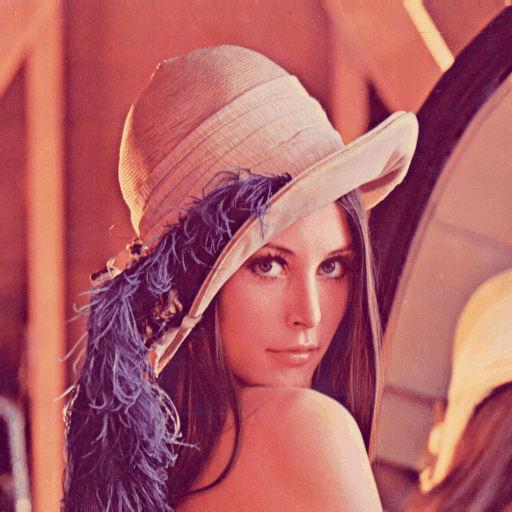
\includegraphics[width=\textwidth]{tex/img/lena.png}
        \caption*{Originale}
      \end{subfigure}
      \hspace{0.15\textwidth}
      \begin{subfigure}[b]{0.33\textwidth}
        \centering
        
\includegraphics[width=\textwidth]{img/lena-threshold-20.png}
        \caption*{\texttt{p }\( = 20\%\)}
      \end{subfigure}

      \vspace{0.02\textwidth}

      \begin{subfigure}[b]{0.33\textwidth}
        \centering
        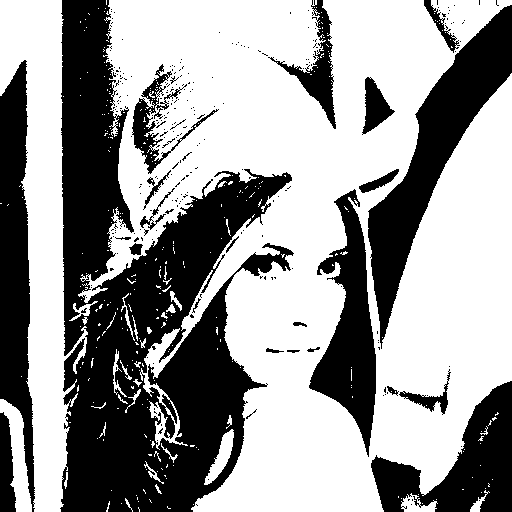
\includegraphics[width=\textwidth]{img/lena-threshold-40.png}
        \caption*{\texttt{p }\( = 40\%\)}
      \end{subfigure}
      \hspace{0.15\textwidth}
      \begin{subfigure}[b]{0.33\textwidth}
        \centering
        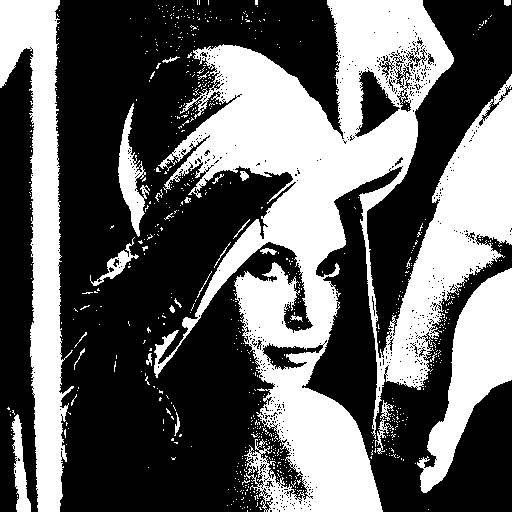
\includegraphics[width=\textwidth]{img/lena-threshold-60.png}
        \caption*{\texttt{p }\( = 60\%\)}
      \end{subfigure}

      \vspace{0.02\textwidth}

      \begin{subfigure}[b]{0.33\textwidth}
        \centering
        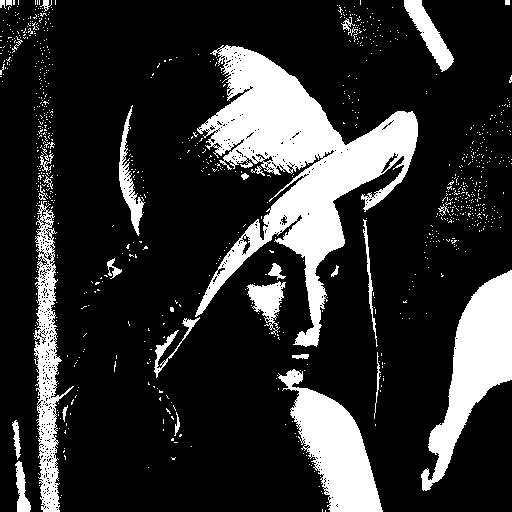
\includegraphics[width=\textwidth]{img/lena-threshold-80.png}
        \caption*{\texttt{p }\( = 80\%\)}
      \end{subfigure}
      \hspace{0.15\textwidth}
      \begin{subfigure}[b]{0.33\textwidth}
        \centering
        
\includegraphics[width=\textwidth]{img/lena-threshold-99.png}
        \caption*{\texttt{p }\( = 99\%\)}
      \end{subfigure}
    \end{figure}

    È inoltre possibile creare, usando l'utility \texttt{convert} di
    ImageMagick, una gif animata i cui frame siano le immagini risultanti
    al variare della soglia da \(0\) a \(99\). Per ottenerla \`e sufficiente
    invocare la rule \texttt{make gif} del \texttt{Makefile} oppure visitare il
    seguente indirizzo: \href{http://raw.github.com/jacquerie/SPM/master/lena.gif}{\underline{http://raw.github.com/jacquerie/SPM/master/lena.gif}}.

  \newpage

  \appendix
    \section{Manuale d'uso}
      \subsection{Makefile}

      \begin{description}
        \item[\texttt{all}:] Invoca le rule \texttt{gif}, \texttt{parallel}, \texttt{sequential} e \texttt{tex}
        \item[\texttt{clean}:] Rimuove i file generati dalle rule \texttt{gif}, \texttt{parallel}, \texttt{sequential} e \texttt{tex}.
        \item[\texttt{gif}:] Genera una gif animata i cui frame sono le
          immagini risultanti al variare della soglia \texttt{p} da \(0\) a
          \(99\). Richiede l'installazione di ImageMagick e che \texttt{convert}
          sia nel \texttt{PATH}.
        \item[\texttt{parallel}:] Compila con \texttt{sketocxx}
          l'implementazione parallela. Richiede l'installazione di SkeTo, una
          distribuzione di MPI compatibile e ImageMagick.
        \item[\texttt{sequential}:] Compila con \texttt{g++} l'implementazione
          sequenziale. Richiede l'installazione di ImageMagick.
        \item[\texttt{tex}:] Compila con \texttt{pdflatex} il presente
          documento. Richiede l'installazione di \texttt{pdflatex} e del
          pacchetto Python \href{http://pygments.org}{\underline{pygments}}.
      \end{description}

      \subsection{Eseguibili}

      \begin{description}
        \item[\texttt{./sequential numberOfJobs}:] Esegue \texttt{sequential}
          su \texttt{numberOfJobs} istanze del problema dell'Histogram
          Thresholding. Stampa su \texttt{stdout} una coppia separata da uno
          spazio in cui il primo numero \`e \texttt{numberOfJobs} e il secondo
          il tempo in secondi impiegato da \texttt{sequential} a meno di
          operazioni di lettura e scrittura sul file system. 
        \item[\texttt{./test\_parallel [numberOfJobs=10]}:] Aggiunge in coda al file
          \texttt{parallel.dat} i risultati di \(10\) invocazioni su \texttt{NP}
          processi, per \texttt{NP} che varia da \(1\) a \(16\),
          dell'implementazione parallela su istanze di taglia
          \texttt{numberOfJobs}. I risultati sono riportati come triple separate
          da spazi in cui il primo numero \`e \texttt{NP}, il secondo
          \texttt{numberOfJobs} e il terzo il tempo impiegato a meno di
          letture e scritture sul file system.
        \item[\texttt{./test\_sequential [numberOfJobs=10]}:] Invoca \(10\)
          volte \texttt{./sequential numberOfJobs} con valore di default \(10\),
          redirigendo \texttt{stdout} sul file \texttt{sequential.dat}.
      \end{description}

      Esiste infine la possibilit\`a di invocare direttamente
      \texttt{./parallel} con la sintassi
      \texttt{sketorun -np NP ./parallel numberOfJobs}, in cui \texttt{NP} \`e
      il numero di processi che si desiderano far partire.

      \subsection{Licenza}

      Il codice \`e rilasciato con \href{http://opensource.org/licenses/MIT}{\underline{licenza MIT}}
      ed \`e disponibile su \href{https://github.com/jacquerie/SPM}{\underline{Github}}.
\end{document}

